%%%%%%%%%%%%Outline%%%%%%%%%%%%%%%%%%

%%% Section 2.1 The eBPF Execution Pipeline

%%%
% message<eBPF execution pipeline overview>
% Figure 1 shows the eBPF execution pipeline
% user-space compiler turns source code into eBPF bytecode
% kernel verifies bytecode, JIT-compiles to native, attaches to hook point
% program runs each time the kernel invokes the hook

%%%
% message<eBPF compilation: source language to bytecode via LLVM>
% eBPF program reaches the kernel as bytecode produced by a user-space compiler
% language-specific front-end lowers source to LLVM IR
% LLVM middle-end runs its optimization passes
% LLVM eBPF backend lowers optimized IR to bytecode, restricted to ISA-defined operations

%%%
% message<verifier: abstract interpretation with per-opcode semantics>
% verifier statically checks safety properties (memory safety, termination, no uninitialized reads)
% method: abstract interpretation
% each of the 117 eBPF ISA opcodes has its own abstract semantics
% unknown opcodes rejected, so adding an opcode requires defining new semantics
% after safety analysis, verifier applies a few targeted bytecode rewrites (DCE, zext insertion)

%%%
% message<JIT: per-instruction translation, encoding-level optimization only>
% JIT translates verified bytecode to native code one opcode at a time
% fixed register mapping
% encoding-level optimizations: shortest immediate, short jumps, callee-saved pruning
% multi-pass convergence until jump encodings stabilize
% no cross-instruction optimization

%%% Section 2.2 The eBPF--Native Performance Gap

%%%
% message<runtime cost from ISA-bounded backend and per-opcode JIT>
% pipeline preserves safety but emits slower native code than direct LLVM compilation
% LLVM eBPF backend cannot emit hardware operations the eBPF ISA does not define
% kernel JIT cannot recover them; each opcode translated independently with encoding-level only
% missing-opcode operations decomposed by backend into multiple eBPF instructions
% JIT translates the decomposed instructions one by one to native
% resulting native sequence longer and slower than direct LLVM x86-64/ARM64 backend

%%%
% message<methodology: measuring the gap with two compilation pipelines>
% to quantify the cost, compile 54 pure-computation eBPF micro benchmarks through two pipelines
% pipeline 1: C to native via LLVM x86-64 backend (upper bound)
% pipeline 2: C to eBPF bytecode via LLVM eBPF backend, then to native via the eBPF JIT
% both pipelines share LLVM front-end and middle-end; only backend target differs

%%%
% message<eBPF JIT 3x slower than native, gap concentrated in specific operation classes>
% 3.0x slower than native, geomean
% category breakdown identifies specific operation classes as primary contributors
% largest per-benchmark slowdowns appear in rotates, endian-aware loads, conditional selects
% next subsection examines one class in detail

%%% Section 2.3 Case Study: The Missing Rotate Opcode

%%%
% message<rotate slowdown traces to a missing opcode, not to JIT quality>
% concrete example: 64-bit rotate-left through both pipelines (figure)
% LLVM x86-64 backend recognizes the rotate idiom and emits a single ROL
% LLVM eBPF backend has no rotate opcode, decomposes into eight eBPF instructions
% eBPF JIT translates each one to one
% same source, compiler, and hardware: the bottleneck is the missing opcode in the eBPF ISA
% per-instruction encoding cannot supply a missing opcode

%%%
% message<rotate is one of five classes of operations the eBPF ISA does not expose>
% rotate is not isolated
% table lists five classes of hardware operations without an eBPF opcode equivalent
% in each class, the eBPF JIT emits a multi-instruction sequence for what hardware does in one or two instructions

%%% Section 2.4 Limitations of Existing Approaches

%%%
% message<pre-load bytecode rewrite cannot supply missing operations>
% one class of approaches rewrites or synthesizes bytecode before kernel load
% no bytecode rewrite can introduce operations the eBPF ISA does not define

%%%
% message<in-kernel extension breaks safety proofs and scales per architecture>
% other class adds richer operations in-kernel: new opcodes, cross-insn JIT transforms, or new verifier passes
% existing formal-verification proofs depend on per-instruction translation and the current per-opcode abstract semantics
% any in-kernel extension invalidates those proofs
% per-opcode engineering also multiplies across architectures (different platforms need different native instructions)
% each new opcode requires backend work in every architecture and upstream kernel review

%%% Section 2.5 Decoupling Verification and Execution

%%%
% message<verification and execution have conflicting demands on a single ISA>
% limitations above share one root: verification and execution conflict on bytecode
% verification needs a simple, architecture-independent representation
% execution needs a richer representation mapping to hardware-specific instructions
% current eBPF design forces both roles onto one ISA, causing the performance gap

%%%
% message<\lang decouples the two with separate representations>
% \lang is extended eBPF bytecode with separate representations for verification and execution
% next chapter describes the design in detail

%%%%%%%%%%%%Outline%%%%%%%%%%%%%%%%%%

% [] zhengjie: original 2.2 and 2.3 move to related work section
% [] zhengjie: 2.1 这里，要讲出现在BPF是在哪里做optimize。还有JIT是1-1翻译，因此verifier验证的程序和实际跑的程序等价，如果JIT正确。而现在已经有工作形式化验证正确性。然后3.2里就可以讲JIT扩充的坏处

\section{Background and Motivation}
\label{sec:background}

This section provides background on eBPF and motivates \lang's design. \S\ref{subsec:ebpf} describes the eBPF execution pipeline. \S\ref{subsec:gap} quantifies the performance gap between eBPF and native code. \S\ref{subsec:approaches} discusses limitations of existing approaches. \S\ref{subsec:insight} states the design insight.

\subsection{The eBPF Execution Pipeline}
\label{subsec:ebpf}

Figure~\ref{fig:ebpf} shows the eBPF execution pipeline. A user-space compiler compiles source code to eBPF bytecode. The kernel then verifies the bytecode, JIT-compiles the verified bytecode to native machine code, and attaches the compiled program to a hook point (e.g., XDP, tc). Once attached, the program runs each time the kernel invokes the hook.

\begin{figure}[t]
  \centering
  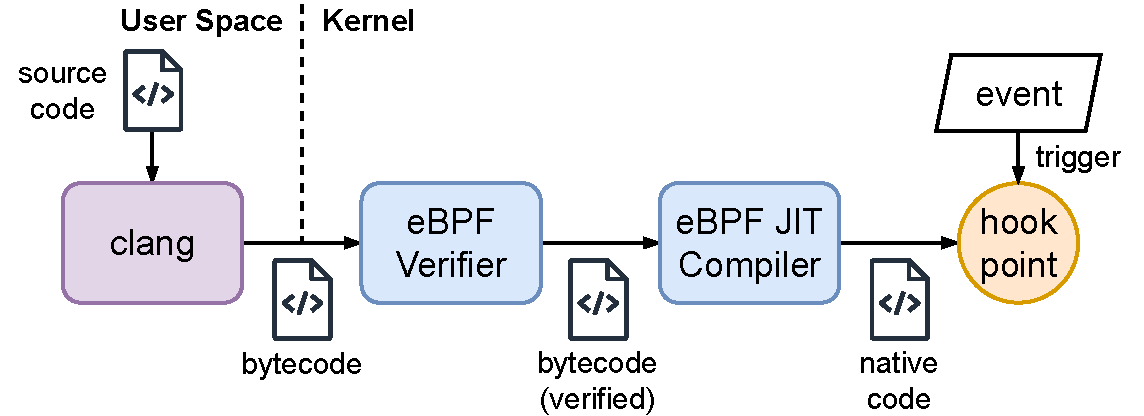
\includegraphics[width=\linewidth]{figures/sec-2-ebpf-pipeline.pdf}
  \caption{The eBPF execution pipeline.}
  \label{fig:ebpf}
\end{figure}

\noindent\textbf{Source compilation.}
An eBPF program reaches the kernel as bytecode produced by a user-space compiler. A language-specific front-end (e.g., Clang for C) lowers source code to LLVM IR. LLVM's middle-end runs its optimization passes. The LLVM eBPF backend lowers the optimized IR to eBPF bytecode, restricted to operations the eBPF ISA defines.

\noindent\textbf{Verification.}
The eBPF verifier statically checks every loaded program for safety, proving properties such as memory safety, termination, and absence of uninitialized reads. The analysis uses abstract interpretation~\cite{gershuni2019simple}. Each of the 117 eBPF ISA opcodes~\cite{rfc9669} has its own abstract semantics. Unknown opcodes are rejected, so adding an opcode requires defining new semantics. After safety analysis succeeds, the verifier also performs a few targeted bytecode rewrites (e.g., dead-code elimination) before passing the program to the JIT.

\noindent\textbf{JIT compilation.}
The eBPF JIT compiler translates the verified bytecode into native machine code. The translation proceeds one instruction at a time, with eBPF registers \texttt{r0}--\texttt{r10} mapped to fixed native registers on each target architecture. Encoding-level optimizations within each instruction include selecting the shortest immediate encoding, choosing short jumps when the offset fits, and emitting prologue push/pop instructions only for callee-saved registers the program uses. Multiple passes iterate until jump encodings stabilize. The JIT performs no cross-instruction optimization (e.g., global register allocation, instruction scheduling).

\subsection{The eBPF-Native Performance Gap}
\label{subsec:gap}

The pipeline above preserves safety but emits slower native code than direct LLVM compilation does. The LLVM eBPF backend cannot emit hardware operations the eBPF ISA does not define. The eBPF JIT compiler cannot recover those operations later, since each opcode is translated independently with only encoding-level optimizations. A hardware operation absent from the eBPF ISA is therefore decomposed by the backend into multiple eBPF instructions. The JIT then translates the decomposed instructions one by one to native. The resulting native sequence is longer and slower than what the LLVM x86-64 or ARM64 backend would emit for the same source.

To quantify the cost, we compile 54 pure-computation eBPF micro benchmarks through two pipelines and compare the results. Each program is compiled (1)~directly from C to native code using LLVM (\texttt{clang} \texttt{-O2}), and (2)~from C to eBPF bytecode using the LLVM eBPF backend, then to native code via the eBPF JIT compiler. Both pipelines use the same LLVM front-end and the same middle-end optimization passes; the only difference is the compilation target.

The eBPF JIT compiler is 3.0$\times$ slower than native on average. Figure~\ref{fig:perf-gap} shows the geometric mean of execution time per category. The gap varies across categories: large programs (4.7$\times$) and dependency chains (4.0$\times$) show the largest gap, while loops (2.1$\times$) show the smallest. Within each category, the largest slowdowns appear in benchmarks that exercise hardware operations absent from the eBPF ISA, such as rotates (5.8$\times$), endian-aware loads (up to 6.6$\times$), and conditional selects (up to 4.1$\times$). \S\ref{subsec:char-rotate} examines these missing operations in detail.

\begin{figure}[t]
\centering
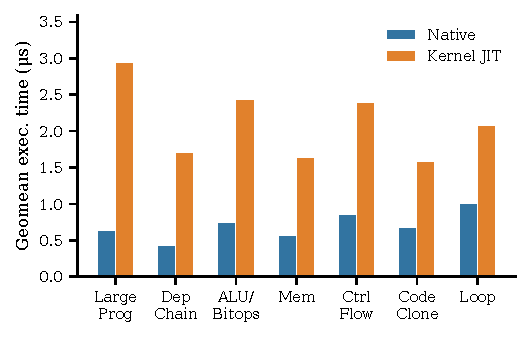
\includegraphics[width=\columnwidth]{figures/sec-3-perf-gap.pdf}
\caption{Geometric mean of execution time per benchmark category for the eBPF JIT compiler relative to native code (LLVM \texttt{-O2}). The 54 benchmarks span seven categories: ALU/bit operations, memory access, control flow, dependency chains, loops, program scale, and code cloning.}
\label{fig:perf-gap}
\end{figure}

\subsection{Limitations of Existing Approaches}
\label{subsec:approaches}

One class of approaches rewrites or synthesizes eBPF bytecode before kernel load~\cite{xu2021synthesizing,mao2024merlin,zhu2025epso}. No such rewrite can introduce operations the eBPF ISA does not define, such as rotate, conditional move, and wide load.

The other class adds richer operations in-kernel: new opcodes to the ISA, cross-instruction transforms to the JIT, or new analysis passes to the verifier. Existing formal-verification proofs~\cite{nelson2020specification} depend on per-instruction translation and the current per-opcode abstract semantics. Any in-kernel extension invalidates these proofs. Per-opcode engineering also multiplies across architectures, since different platforms need different native instructions for the same operation (x86 \texttt{ROL} vs.\ ARM64 \texttt{ROR}). Each new opcode therefore requires backend work in every architecture and upstream kernel review.

\subsection{Decoupling Verification and Execution}
\label{subsec:insight}

The limitations above share a common root: verification and execution make conflicting demands on the bytecode. Verification needs a simple, architecture-independent representation that the existing verifier accepts. Execution needs a richer representation that maps to hardware-specific instructions the eBPF JIT compiler can emit directly. The current eBPF design forces both roles onto a single ISA, causing the performance gap.

To decouple these two roles, we introduce \lang, an extended eBPF bytecode that uses separate representations for verification and execution. \S\ref{sec:design} describes the design.
